\documentclass[12pt]{article} \usepackage{url, graphicx}

% page layout
\setlength{\topmargin}{-0.25in}
\setlength{\textheight}{9.5in}
\setlength{\headheight}{0in}
\setlength{\headsep}{0in}

% problem formatting
\newcommand{\problemname}{Problem}
\newcounter{problem}

% math
\newcommand{\dd}{\mathrm{d}}

% primary units
\newcommand{\rad}{\mathrm{rad}}
\newcommand{\kg}{\mathrm{kg}}
\newcommand{\m}{\mathrm{m}}
\newcommand{\s}{\mathrm{s}}

% secondary units
\renewcommand{\deg}{\mathrm{deg}}
\newcommand{\km}{\mathrm{km}}
\newcommand{\mi}{\mathrm{mi}}
\newcommand{\h}{\mathrm{h}}
\newcommand{\ns}{\mathrm{ns}}
\newcommand{\J}{\mathrm{J}}
\newcommand{\eV}{\mathrm{eV}}
\newcommand{\W}{\mathrm{W}}

% derived units
\newcommand{\mps}{\m\,\s^{-1}}
\newcommand{\mph}{\mi\,\h^{-1}}
\newcommand{\mpss}{\m\,\s^{-2}}

% random stuff
\sloppy\sloppypar\raggedbottom\frenchspacing\thispagestyle{empty}

\begin{document}

\noindent
Name: \rule[-1ex]{0.55\textwidth}{0.1pt}
NetID: \rule[-1ex]{0.2\textwidth}{0.1pt}

\section*{NYU Physics I---Final Exam}

\paragraph{\problemname~\theproblem:}\refstepcounter{problem}%
If a car gets 20 miles to the gallon, how many liters of fuel
does it take to go 100 km? A gallon is about 4 liters, and a mile is
about 1.6 km.
(From Problem Set 1.)

\vfill

\paragraph{\problemname~\theproblem:}\refstepcounter{problem}%
Consider a stone thrown (at $t=0$) precisely upwards (in the $y$
direction, for definiteness) at $1.0\,\m\,\s^{-1}$, with an initial
position (launch point) at $y=0$.  Ignore air resistance! Make one
very careful plot of the vertical velocity $v_y$ of the stone as a
function of time $t$ for the duration $0<t<0.3\,\s$. Use
$g=10\,\m\,\s^{-2}$.
(From Problem Set 2.)

\vfill

\paragraph{\problemname~\theproblem:}\refstepcounter{problem}%
foo

\vfill
~
\clearpage

\paragraph{\problemname~\theproblem:}\refstepcounter{problem}%
Draw the free-body diagram for the pulley in this device.
(From Problem set 3.)\\
~\hfill\includegraphics{../mp/pulley_table.pdf}\hfill~

\vfill

\paragraph{\problemname~\theproblem:}\refstepcounter{problem}%
foo

\vfill

\paragraph{\problemname~\theproblem:}\refstepcounter{problem}%
You have a block of mass $m$ on an inclined
plane, inclined at an angle $\theta=15\,\deg$ to the horizontal. The
coefficient of friction is $\mu=0.5$. What is the magnitude of the
frictional force on the block? The acceleration due to gravity is $g$.
Once again, state any assumptions you need to make.
(From friction worksheet.)

\vfill
~
\clearpage

\paragraph{\problemname~\theproblem:}\refstepcounter{problem}%
What is the power output (energy per time) for a normal, healthy NYU
student climbing stairs at a typical pace? Compute only the
potential-energy work; don't consider metabolic losses or kinetic
energy.
(From Problem Set 4.)

\vfill

\paragraph{\problemname~\theproblem:}\refstepcounter{problem}%
foo

\vfill

\paragraph{\problemname~\theproblem:}\refstepcounter{problem}%
An elastic ball of mass $m$ heads at speed $v$ towards a huge wall.
Its initial velocity is at an angle of $\theta$ to the normal.
Imagine that the collision is perfectly elastic and the
wall is perfectly frictionless, so the ``angle of incidence equals the
angle of reflection''. What is the magnitude of the momentum change of the ball (final
minus initial)?
Give your answer in terms of the symbols in the diagram.
(from bouncing worksheet.)
\marginpar{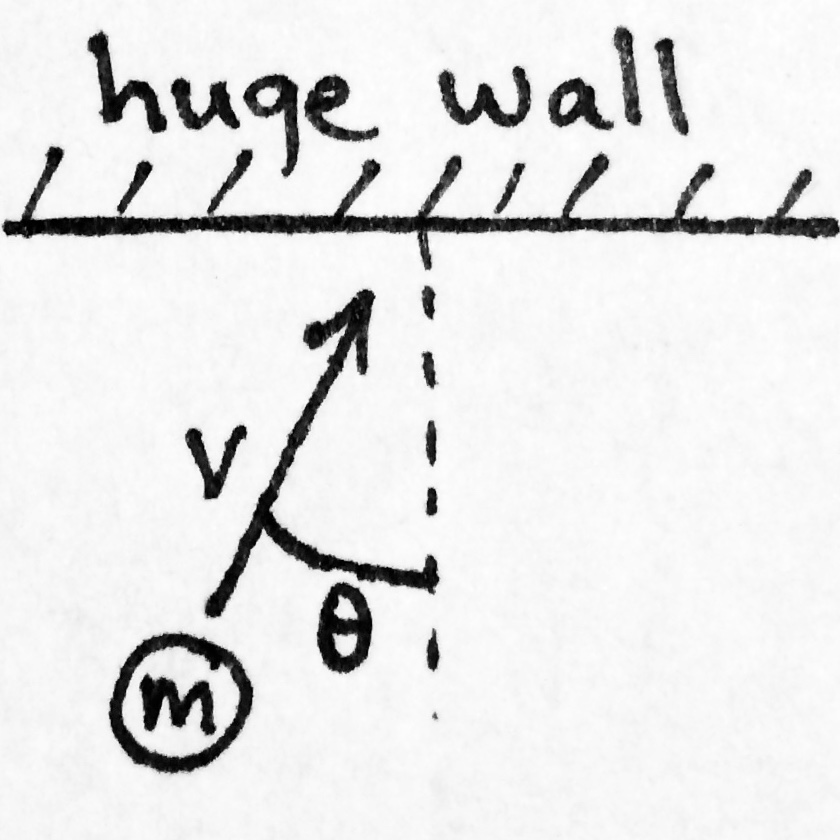
\includegraphics[width=1in]{../jpg/ballwall.jpg}}

\vfill
~
\clearpage

\paragraph{\problemname~\theproblem:}\refstepcounter{problem}%
A student of mass $m_\mathrm{student}=80\,\kg$ stands at rest next to
a block of ice of mass $m_\mathrm{ice}=320\,\kg$, also at rest, on a
frictionless frozen lake.  The student pushes on the block until the
block is moving away from the student at $1.5\,\mps$ (that is, until
$\left|\vec{v}_\mathrm{ice}-\vec{v}_\mathrm{student}\right|=1.5\,\mps$).
What is the total momentum of the student-plus-block system after the
push? That is, after they are both moving?
(From Problem Set 5.)

\vfill

\paragraph{\problemname~\theproblem:}\refstepcounter{problem}%
foo

\vfill

\paragraph{\problemname~\theproblem:}\refstepcounter{problem}%
A block of mass $4\,\kg$ is moving in the positive $x$ direction at
$1\,\mps$, and a block of mass $6\,\kg$ is moving in the negative $x$ direction
at $2\,\mps$. What is the velocity (magnitude and direction) of the
center of mass of the two-block system?
(From Problem Set 6.)

\vfill
~
\clearpage

\paragraph{\problemname~\theproblem:}\refstepcounter{problem}%
What are the units of $P\,V$ (that is, pressure times volume)?
(From worksheet on the ideal gas.)

\vfill

\paragraph{\problemname~\theproblem:}\refstepcounter{problem}%
foo

\vfill

\paragraph{\problemname~\theproblem:}\refstepcounter{problem}%
You calculated that a pendulum with a period of $2\,\s$ has a length
very close to $1\,\m$. What would be the length of a pendulum with
a period of $8\,\s$? (From Problem Set 7.)

\vfill
~
\clearpage

\paragraph{\problemname~\theproblem:}\refstepcounter{problem}%
A very thin ladder of length $L$ and mass $M$ leans against a vertical
wall, on a horizontal floor, making a small angle of $\theta$ with respect
to the wall.  Imagine that there is a large coefficient of friction
$\mu$ at the floor so that the ladder is in static
equilibrium, but assume that the wall is effectively frictionless.
Draw a free-body diagram for the ladder, showing all
forces acting.
(From Problem Set 8.)

\vfill

\paragraph{\problemname~\theproblem:}\refstepcounter{problem}%
foo

\vfill

\paragraph{\problemname~\theproblem:}\refstepcounter{problem}%
In a piano, each string has a mass $M$, a length $L$, and a tension $T$.
Use dimensional analysis to estimate the natural angular
frequency $\omega$ of a piano string with these properties. That is,
what combination has units of frequency?
(From Problem Set 9.)

\vfill
~
\clearpage

\paragraph{\problemname~\theproblem:}\refstepcounter{problem}%
Immediately after being hit, at $t=0$, a cue ball of mass
$M$ and radius $R$ slides along the felt at speed $v_i$, not rotating
at all.
Assume that there is a
coefficient $\mu$ of sliding friction.
What is the torque on the cue ball? Be sure to specify your reference point or axis!
(From Problem Set 10.)

\vfill

\paragraph{\problemname~\theproblem:}\refstepcounter{problem}%
Which is bigger in magnitude? The angular momentum from the fact
that the Earth is spinning around its own axis? Or the angular
momentum from the fact that the Earth is going around the Sun?
(From Problem Set 11.)

\vfill

\paragraph{\problemname~\theproblem:}\refstepcounter{problem}%
If the Earth were half as massive as it is, but were still
on a near-circular orbit at its current Earth--Sun distance, how much
longer or shorter would the year be?
(From the recitation on orbits.)

\vfill
~
\clearpage

\paragraph{\problemname~\theproblem:}\refstepcounter{problem}%
Sketch Solar-System orbits of fixed semi-major axis but increasing
eccentricity, from a circular orbit, to one that is close to radial
(eccentricity close to unity). Make sure you show the position of
the Sun inside each orbit.
(From Problem Set 12.)

\vfill

\paragraph{\problemname~\theproblem:}\refstepcounter{problem}%
How long does it take light to go $1\,\ft$?
(From Problem Set 13.)

\vfill

\paragraph{\problemname~\theproblem:}\refstepcounter{problem}%
One sibling (homebody) lives at home, and the other (traveler) is
traveling away from home at dimensionless speed $\beta$. The traveler
is sending, by radio transmission, a birthday greeting home every year
(according to her). What is the time separation between these
greetings as they are received by the homebody, according to the
traveler?
(From Problem Set 14.)

\vfill
~
\end{document}
